\section{Anwendung der Testgetriebenen Entwicklung am Beispiel einer Stellenanzeige}
In den nachfolgenden Abschnitten wird examplarisch die Domäne "`Job"' der Webanwendung näher erläutert werden
    
    
\subsection{Implementierung von Unit-Tests}    

Ein Modell repräsentiert die Daten der Anwendung, und die Regeln, wie diese zu verändern sind. Bei Rails werden sie hauptsächlich dazu verwendet, um mit der zugrundeliegenden Datenbanktabelle zu interagieren. Per Konvention von Rails findet hier die Hauptarbeit, also die Business-Logik, statt.

Fast jeder Unittest bei Rails überprüft Validierungskritieren seines korrespondierenden Modells, d.h. wann eine Instanz dieses Modells gültig ist und damit gespeichert werden darf (man denke z.B. an Pflichtfelder für ein Modell "`Nutzer"` oder die Validierung des Formates seiner E-Mail-Adresse). Daneben sollten natürlich alle weiteren, selbstdefinierten, Methoden getestet werden.
% TODO http://guides.rubyonrails.org/getting_started.html#the-mvc-architecture

\paragraph{1. Der Anfang}

Während der Analyse wurden die wahrscheinlich benötigten Attribute bestimmt. In Abbildung \ref{fig:job-erm} seien die Basisattribute der Tabelle dargestellt. Neben den einfachen Attributen, wie Title, Description und Link, existieren auch Referenzen auf andere Objekte (d.h. dies stellen Fremdschlüssel zu anderen Tabellen dar), wie z.B. Schlagwörter (Tags), ein Besitzer einer Stellenanzeige (User) und so weiter.

\begin{figure}[h]
 \centering
 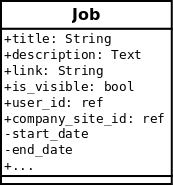
\includegraphics{../diagrams/job-erm.png}
 % job-erm.png: 173x186 pixel, 51dpi, 8.65x9.30 cm, bb=0 0 245 264
 \label{fig:job-erm}
 \caption{Attribute des Modells "'Job"`}
\end{figure}

In der Regel erfolgt nun eine Generation der Testklasse und des Testmodells mittels der mitgelieferten Codegeneratoren. 
\begin{lstlisting}
~/it-jobs$ rails generate model job title:string link:string \
    description:text user:references visible:boolean ...

      invoke  active_record
      create    db/migrate/20110828160636_create_jobs.rb
      create    app/models/job.rb
      invoke    test_unit
      create      test/unit/job_test.rb
      create      test/fixtures/jobs.yml

\end{lstlisting}
Mit der Anweisung uns ein Modell "'job"` mit den nachfolgenden Attributen zu generieren, hat Rails uns nun schon ein Stück Arbeit abgenommen. Es wurden erstellt:
\begin{itemize}
 \item Eine Migration (\verb|db/migrate/2011xxxxxx_create_jobs.rb|). Dies stellt eine datenbankunabhängige Repräsentation einer Änderung an der Struktur unserer Datenbank dar. In diesem ist es die Erstellung einer Tabelle "'jobs"` (beachte: Plural!)
 \item Die Modelklasse (\verb|app/models/job.rb|)
 \item Die dazugehörige Testklasse (\verb|app/unit/job_test.rb|)
 \item und Fixtures-Datei (\verb|test/fixtures/jobs.yml|), zur Definition von Testdaten. 
\end{itemize}


Nach einer Erstellung der (SQLite)-Datenbank und Ausführung der Migration kann die Rails-Test-Suite nun auch schon ausgeführt werden:

\begin{lstlisting}
$ rake db:migrate && rake test
 
==  CreateJobs: migrating =====================================================
-- create_table(:jobs)
   -> 0.0020s
==  CreateJobs: migrated (0.0021s) ============================================

(in /home/zealot64/TEST)
Loaded suite /usr/lib/ruby/gems/1.8/gems/rake-0.8.7/lib/rake/rake_test_loader
Started
.
Finished in 0.043818 seconds.

1 tests, 1 assertions, 0 failures, 0 errors

\end{lstlisting}

Es wurde also schon ein Testfall erfolgreich ausgeführt, nämlich ein Dummytestfall von Rails:

\begin{lstlisting}
test/unit/job_test.rb 
require 'test_helper'

class JobTest < ActiveSupport::TestCase
  # Replace this with your real tests.
  test "the truth" do
    assert true
  end
end
\end{lstlisting}



TODO 

* Test ob ein Nutzer einen Titel braucht
* Testen des Formats der E-Mail Adresse




\paragraph{Refaktorisierungen der Testklasse}


\begin{lstlisting}
 %jobs.yml
first_job:
  title: Ruby on Rails Entwickler
  description: Lorem ipsum dolor sit...
  link: http://www.example.com/job/123
  visible: true
  user_id: 1
non_visible_job:
  visible: false
  ...
\end{lstlisting}

Damit verkürzt sich die Initialisierung auf das Laden der Fixture mit dem Namen "'test\_job"`.

\begin{lstlisting}
class JobTest < ActiveSupport::TestCase
  setup do
    @job = jobs(:test_job)
  end

  test "Factory sollte gültige Jobs generieren" do
    assert_save @job
  end
end
\end{lstlisting}


\subsection{Implementierung von Controller-Tests (functional tests)}

Neben den Unittests stellt Ruby on Rails eine weitere Testart nativ bereit. Dies sind die sogenannten Functional Tests, deren Testobjekt ein Controller ist. Dieser ist ein abgeschlossenes Objekt, was functional tests damit letztendlich nur zu einer Variation des Unittest macht.
Ein Controller hat bei Ruby on Rails die Aufgabe, Anfragen für bestimmte Routen, also Web-Adressen, anzunehmen, die Arbeit an eine Modelklasse auszulagern, und eine View aufzurufen, die letztendlich HTML-Code generiert.
    
    
\subsection{Testen von externen Zugriffen mittels Mocks und Stubs am Beispiel Feedimport}


\subsection{Testen von Javascript Ereignissen}

Unittests:  Jasmine fuer komplexe Objekte und Javascript Anwendungen

Systemtests mittels Selenium fuer vereinzeltes JS in Form von


